%------------------------------------------------
% Quick reference. 
%------------------------------------------------
%
% Для вставки картинок:
%
%--------         Комманда
%
%\begin{figure}[H]
%	\includegraphics{img_name}
%	\caption{some caption}
%	\label{some_pic}
%\end{figure}
%
%--------        Переменные
%
% img_name     <- Название картинки в папке img.
% some_caption <- подпись картинки.
% label        <- лейбл нужен для ссылок на картинку.
% H            <- расположение картинки на странице.
%
%--------         Пример
%
%\begin{figure}[H]
%	\includegraphics{pic1.jpg}
%	\caption{График зависимости чего-то там}
%	\label{grapics1}
%\end{figure}
%
%------------------------------------------------
%
% Для референса по лейблу:
%
%--------         Комманда
%
% Для ссылки используется \eqref{ref}.
%
%--------        Переменные
%
% ref          <- указанный лейбл в директиве \label{ref}
%                 Ссылку можно сделать на любой объект имеющий \label{•}
%
%--------         Пример
%
% \eqref{graphics1}
%
% Ссылка на источники [\ref{src_spectral_wiki}]
%
%------------------------------------------------
%
% Для листинга кода:
%
%--------         Комманда
%
% \lstinputlisting[language=lang,mathescape=true]{src}
%--------        Переменные
%
% lang         <- язык на котором написан исходный код, например "python" или "C++".
% mathescape   <- если в исходниках есть формулы LaTeX, то они будут представлены как формулы.
% src          <- путь до файла исходников.
%
%--------         Пример
%
% \lstinputlisting[language=C++,mathescape=false]{./src/bullshit.cpp}
%
%------------------------------------------------
%
% Для вставки таблиц:
%
%--------
%\begin{table}[H]
%	\centering
%	\caption{ capt }
%	\begin{tabularx}{0.9\textwidth}{ | Y | Y | }
%		\hline
%		lines
%	\end{tabularx}
%	\label{tab1}
%\end{table}
%--------
% caption      <- Подпись таблицы.
% tab1         <- лейбл нужный для ссылки на таблицу.
% | Y | Y |    <- количество и формат столбцов.
% Y            <- Тип столбца.
%                 В данном случае определены кастомные столбцы Y (Спасибо Максиму Наумову)
% |            <- обозначает границы столбца.
%                 То есть, если будет указано |Y Y|, то столбцы внутри строк разделены не будут.
% H            <- То же самое, что и у картинок.
% lines        <- непосредственно элементы таблицы.
%                 Разделяются знаком "&", оканчивать каждую строку лучше \\ \hline
%
%--------         Пример
%\begin{table}[H]
%	\centering
%	\caption{ capt }
%	\begin{tabularx}{0.9\textwidth}{ | Y | Y | }
%		\hline
%		str1 & str2 \\ \hline
%		str1 & str2 \\ \hline
%		str1 & str2 \\ \hline
%		str1 & str2 \\ \hline
%		str1 & str2 \\ \hline
%	\end{tabularx}
%	\label{tab1}
%\end{table}
%------------------------------------------------

\documentclass[14pt, a4paper, fleqn]{extarticle}

\makeatletter
\renewcommand*\l@section{\@dottedtocline{1}{1.5em}{2.3em}}



%\includegraphics{universe}

\usepackage[utf8]{inputenc}
\usepackage[T2A]{fontenc}
\usepackage[russian]{babel} % указывает язык документа
\usepackage[left=3cm,right=2cm,top=2cm,bottom=2cm,bindingoffset=0cm]{geometry}
\usepackage{lastpage}
\usepackage{fancyhdr}
\usepackage{titlesec}
\usepackage{multirow}
\usepackage{graphicx} % для вставки картинок
\usepackage[intlimits]{mathtools} % математические дополнения
\usepackage{amssymb}
\usepackage[tableposition=top]{caption}
\usepackage{subcaption}
\usepackage{indentfirst}
\usepackage{pythonhighlight}
\usepackage{listings}
\usepackage{tabularx}
\usepackage{tabulary}
\usepackage{multirow}
\usepackage{xcolor,colortbl}
\usepackage{float}
\usepackage[figure,table]{totalcount}
\usepackage{diagbox}
\usepackage[german=guillemets]{csquotes}
\usepackage{fontspec} 
\usepackage{enumitem}
%\usepackage{mathptmx}% http://ctan.org/pkg/mathptmx
%\usepackage{showframe}
\usepackage{hyperref}

\setlength{\parindent}{1.2cm}

\setlength{\mathindent}{1.2cm}

\defaultfontfeatures{Ligatures={TeX},Renderer=Basic} 
\setmainfont[Ligatures={TeX,Historic}]{Times New Roman}

%\setlist[enumerate]{itemindent=\dimexpr\labelwidth+\labelsep\relax,leftmargin=0pt}

%\setlength{\section*}{0.5cm}
%\usepackage{minted}
%\usepackage{fancyvrb}
%\usepackage{newtxtext}

%\titleformat{\section}[hang]{\bfseries\LARGE\centering}{}{1em}{}

%\setlist[enumerate]{itemindent=\dimexpr\labelwidth+\labelsep\relax,leftmargin=0pt}
\setlist[enumerate,itemize]{leftmargin=0pt,itemindent=1.7cm}
\titlespacing*{\section}{0.6cm}{1ex}{1em}
\titleformat{\section}{\bfseries\centering}{\thesection}{0.5em}{\MakeUppercase}
\titleformat{\subsection}[block]{\bfseries\hspace{1em}}{\thesubsection}{0.5em}{}
%\setlength{\subsection*}{1.5cm}
%\setlength{\parindent}{4em}

%\setlength{\parindent}{1.5cm}

\captionsetup[figure]{name={Рисунок},labelsep=endash, skip=5pt}
\captionsetup[table]{name={Таблица},labelsep=endash,singlelinecheck=false, skip=5pt}


%\renewcommand{\baselinestretch}{1.5}
\linespread{1.5} % полуторный интервал
\frenchspacing
\graphicspath{ {images/} }

%-------------------------------------------
% Ссылки в оглавлении
%-------------------------------------------

\hypersetup{
    colorlinks,
    citecolor=black,
    filecolor=black,
    linkcolor=black,
    urlcolor=black
}

%-------------------------------------------
% Стиль футеров и хедеров
%-------------------------------------------

\pagestyle{fancy}
\fancyhead[L, R]{}
\fancyfoot[L]{}
\fancyfoot[R]{}
\renewcommand{\footrulewidth}{0pt}
\renewcommand{\headrulewidth}{0pt}

%\renewcommand\subsectionfont{\normalfont\normalsize\bfseries}

\def\l@subsection{\@dottedtocline{2}{3.8em}{3.2em}}
\setcounter{tocdepth}{2}
% Для листинга

\lstset{
basicstyle=\footnotesize\ttfamily,
columns=fullflexible,
keywordstyle=\color{blue},
%frame=single,
breaklines=true,
numberstyle=\tiny\color{mygray},
postbreak=\mbox{\textcolor{red}{$\hookrightarrow$}\space},
showstringspaces=false,
}

\newcolumntype{Y}{>{\centering\arraybackslash}X}

%\renewcommand{\theenumi}{\the}
\newcommand{\incpic}[3]{
	\begin{figure}[H] 
		\begin{center} 
			\includegraphics[height=0.6\textwidth]{#1} 
			\caption{#2}
			\label{#3} 
		\end{center}
	\end{figure} 
}

\begin{document}

\pagenumbering{arabic}

\setcounter{page}{3}
%\setcounter{tocdepth}{3}
\setcounter{secnumdepth}{3}

%------------------------------------------------
% Реферат
%------------------------------------------------
\phantomsection
\section*{РЕФЕРАТ}
{
	{\bf Отчет:}
	\pageref{LastPage} страниц,
	%42 страницы,
	\totalfigures\ рисунков,
%	\totaltables\ таблицы,
	13 источников.
%	1 приложение.
	
	%{\bf Презентация:} 19 страниц PDF.\\
	
	\textit{ОБРАБОТКА ИЗОБРАЖЕНИЙ, ДЕСКРИПТОРЫ ТОЧЕК, DAISY, \\SIFT, SURF, PYTHON.}\\
	
	В данной работе рассмотрены алгоритмы построения дескрипторов в задачах обработки изображений.
	
	Цель работы -- разработка устойчивого к пространственным преобразованиям алгоритма построения дескрипторов.
	
	Рассмотрены принципы построения дескрипторов изображений, создана программная реализация с применением алгоритма DAISY, проведено экспериментальное исследование работы алгоритма.
}
\newpage

\newpage
\tableofcontents


%------------------------------------------------
% Введение
%------------------------------------------------
\newpage
\phantomsection
\addcontentsline{toc}{section}{Введение}
\section*{Введение}
{	
	В ряде задач цифровой обработки изображений возникает необходимость однозначного численного описания представленных на изображении точек. В частности, на численном описании отдельных точек и областей изображения основаны решения задач идентификации объектов, совмещения изображений, построения карт глубины и восстановления трехмерной сцены методами фотограмметрии, и многих других.
	
	Математические объекты, описывающие точку изображения, называют дескрипторами. Существует значительное число алгоритмов построения дескрипторов, отличающихся деталями своей реализации, скоростью и точностью работы, а также корректностю результатов для различных исходных данных. 
	
	Основными требованиями к дескриптору являются однозначность результата для одинаковых точек изображений, устойчивость к пространственным и яркостным преобразованиям исходных данных, а также вычислительная сложность алгоритмов построения. 
	
	Целью работы является разработка дескриптора изображений, устойчивого к пространственным преобразованиям.
	
	В данной работе были рассмотрены некоторые дескрипторы и алгоритмы их построения, методы программной реализации. Разработана реализация построения дескрипторов на основе алгоритма DAISY.  
	
	Используемые алгоритмы реализованы на языке программирования общего назначения Python 3.7 с использованием open-source библиотек для обработки изображений OpenCV версии 3.4.2 и scikit-image версии 0.6.12. В качестве тестовых данных использовались наборы изображений из ряда открытых источников.
}

\newpage

%------------------------------------------------
% Начало основной части
%------------------------------------------------
%\titleformat{\section}[runin]{\bfseries\RaggedRight\nohyphens}{\thesection}{0.5em}{}{}
\titleformat{\section}[block]{\bfseries\hspace{0.2em}}{\thesection}{0.5em}{}{}
\titleformat{\subsection}[block]{\bfseries\hspace{1.2em}}{\thesubsection}{0.5em}{}
\titleformat{\subsubsection}[block]{\bfseries\hspace{1.2em}}{\thesubsubsection}{0.5em}{}
\titlespacing*{\section}{1.1cm}{1ex}{1em}
\titlespacing*{\subsection}{0.6cm}{1ex}{1em}
\titlespacing*{\subsubsection}{0.6cm}{1ex}{1em}
\section{Исследование алгоритмов построения дескрипторов изображений}
{
\subsection{Постановка задачи}{
	Дескриптором называют математический объект, сопоставленный с определенной точкой изображения, и представляющий достаточно однозначное ее описание, позволяющее с высокой степенью уверенности идентифицировать аналогичную точку или область на другом изображении. 
	
	Как правило, дескриптор представляет собой вектор значений, вычисляемый определенной функцией для точки изображения.
	
	Стоит заметить, что на практике для однозначного описания точки изображения недостаточно исключительно информации о яркости отдельного пикселя. В связи с этим, в качестве исходных данных для построения дескриптора используется набор из нескольких точек изображения, находящихся в окрестности заданной.  
	
	Рассмотрим следующую постановку задачи.
	Обозначим дескриптор точки $p$ как $d_p$.
	Пусть дано изображение:
	\begin{equation}\label{problem_images}
	I : S \rightarrow \mathbb{R}, \quad S \subset \mathbb{R}^k,
	\end{equation}
	   	\begin{tabular}{ rl }
	  	 \quad \quad где 
	   	& $k$ -- размерность, для плоских изображений равная 2.
	   	\end{tabular}\\
   
	Построение дескриптора будет выглядеть следующим образом:
	\begin{equation}\label{problem_transform}
	d_p = f(I(\hat{p})), \quad \hat{p} \in S.
	\end{equation} 
	   	\begin{tabular}{ rl }
	   	\quad \quad где 
	   	& $f$ -- функция построения дескриптора, \\
	   	& $\hat{p}$ -- набор точек изображения $I$.
	\end{tabular}\\

	Данная схема сохраняется независимо от конкретного алгоритма построения дескриптора. Конкретный вид и свойства полученного результата будут зависеть как от вида функции $f$, так и от конфигурации набора исходных точек $\hat{p}$.
 
	Основным требованием к дескриптору является однозначность результата, т.е. удовлетворение значения \eqref{problem_transform}  следующему выражению для произвольного числа изображений $N$:
	\begin{equation}\label{problem_constraints}
	f(I_i(\hat{p_i})) = f(I_j(\hat{p_j})), \quad i=1 \hdots N, \quad j=1 \hdots N,
	\end{equation} 
	\begin{tabular}{ rl }
	\quad \quad где 
	& $p_i, p_j$ -- пара соответствующих точек изображений $I_i$, $I_j$.
	\end{tabular}\\

	Следует заметить, что построенные дескрипторы, как правило, подвергаются нормализации для уменьшения влияния на точность идентификации точек яркостных характеристик изображения и пространственных преобразований. Конкретные методы нормализации будут рассмотрены в следующих разделах. 
	
	Таким образом, используя различные функции построения и варьируя набор исходных точек, можно получать дескрипторы, обладающие различными свойствами, достоинствами и недостатками для конкретных задач. 
	
	Основными факторами, принимаемыми в расчет при разработке алгоритма построения дескрипторов, являются:
	\begin{enumerate}
	   	\item Устойчивость к пространственным преобразованиям - сохранение значения дескриптора при повороте, сдвиге, масштабировании изображения;
	   	\item Устойчивость к яркостным преобразованиями - сохранение значения дескриптора при изменении яркости и контрастности;
	   	\item Вычислительная сложность построения;
	   	\item Информативность - достаточность данных дескриптора для дальнейшей идентификации и сравнения точек.
	\end{enumerate} 
	
	Следует отметить разницу в требованиях к алгоритму построения дескрипторов в зависимости от предметной области применения. В случае использования дескрипторов для описания особых точек (features) необходима повышенная точность идентификации и инвариантность к преобразованиям, вычислительная сложность же не является самым важным критерием, т.к. число особых точек на изображении, как правило, на порядки меньше его размерности. 
	
	Напротив, в задачах плотного сопоставления изображений, возникающих в фотограмметрии и построении карт глубины, требуется вычисление дескриптора для каждого пикселя, что накладывает дополнительные ограничения на вычислительную сложность. При этом точностью построения и идентификации возможно в некоторой степени пренебречь, т.к. в данных задачах дескрипторы применяются для оценки общих тенденций преобразований между изображениями, что позволяет за счет их большого количества добиться хороших результатов усреднением и дополнительной валидацией.
	
	Существует значительное число реализаций алгоритмов построения дескрипторов. Далее будут рассмотрены некоторые популярные методы и их особенности.
	
\newpage
\subsection{Существующие методы построения дескрипторов}{
	
	\subsubsection{SIFT}{
	Большинство существующих дескрипторов основаны на методах сбора информации о градиенте освещенности изображения в некоторой локальной окрестности точки. 
	Распространенным решением для построения дескрипторов является алгоритм SIFT. 
	
	В методе SIFT дескриптором является вектор. Как и направление ключевой точки, дескриптор вычисляется на гауссиане, ближайшем по масштабу к ключевой точке, и исходя из градиентов в некотором окне ключевой точки. Перед вычислением дескриптора это окно поворачивают на угол направления ключевой точки, чем и достигается инвариантность относительно поворота.
	
	\begin{figure}[H]
		\centering                             
		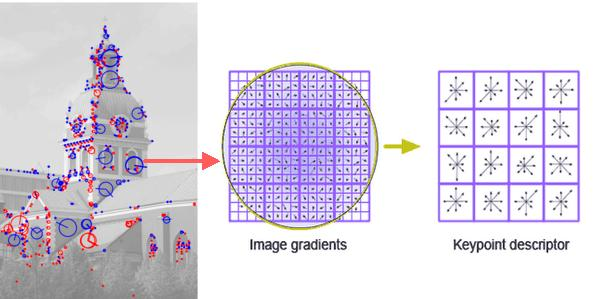
\includegraphics[width=0.6\textwidth,keepaspectratio]{daisy/SIFT.jpg}       
		\centering\caption{ Построение дескриптора SIFT }
		\label{gradient_example}                           
	\end{figure}    
	
	Дескриптор точки состоит из всех полученных гистограмм в ее локальной окрестности. На практике используются дескрипторы размерности 128 компонент (4x4x8).
	
	Полученный дескриптор нормализуется, после чего все его компоненты, значение которых больше 0.2, урезаются до значения 0.2 и затем дескриптор нормализуется ещё раз. В таком виде дескрипторы готовы к использованию.
	
	Существует большое число модификаций SIFT, направленных на улучшение устойчивости к определенным преобразованиям. 
	}
	\subsubsection{SURF}{
	Дескриптор SURF (Speeded up Robust Features) относится к числу тех дескрипторов, которые одновременно выполняют поиск особых точек и строят их описание, инвариантное к изменению масштаба и вращения. Кроме того, сам поиск ключевых точек обладает инвариантностью в том смысле, что повернутый объект сцены имеет тот же набор особых точек, что и образец.
	
	\begin{figure}[H]
		\centering                             
		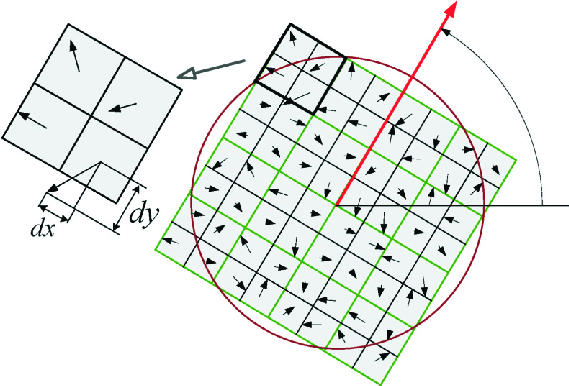
\includegraphics[width=0.6\textwidth,keepaspectratio]{daisy/SURF.png}       
		\centering\caption{ Построение дескриптора SURF }
		\label{gradient_example}                           
	\end{figure}    
	
	Определение особых точек на изображении выполняется на основании матрицы Гессе. Использование Гессиана обеспечивает инвариантность относительно преобразования типа "поворот", но не инвариантность относительно изменения масштаба. Поэтому SURF применяет фильтры разного масштаба для вычисления Гессиана. Для каждой найденной особой точки вычисляется ориентация – преобладающее направление перепада яркости. Понятие ориентации близко к понятию направления градиента, но для определения ориентации особой точки применяется фильтр Хаара. Дескриптор формируется в результате склеивания взвешенных описаний градиента для 16 квадрантов вокруг особой точки. Элементы дескриптора взвешиваются на коэффициенты Гауссова ядра. Веса необходимы для большей устойчивости к шумам в удаленных точках.
	}

	\subsubsection{GLOH}{
	Дескриптор GLOH (Gradient location-orientation histogram) является модификацией SIFT-дескриптора, который построен с целью повышения надежности. Вычисляется SIFT дескриптор, но используется полярная сетка разбиения окрестности на бины: 3 радиальных блока с радиусами 6, 11 и 15 пикселей и 8 секторов. В результате получается вектор, содержащий 272 компоненты, который проецируется в пространство размерности 128 посредством использования анализа главных компонент (PCA).	
	
	\begin{figure}[H]
		\centering                             
		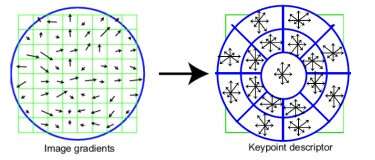
\includegraphics[width=0.6\textwidth,keepaspectratio]{daisy/GLOH.jpg}       
		\centering\caption{ Построение дескриптора GLOH }
		\label{gradient_example}                           
	\end{figure} 

	Общим для всех описанных алгоритмов является основанность на механизмах расчета локального градиента. Данный процесс, несмотря на высокую точность, может быть достаточно вычислительно сложным, что в особенности проявляется в задачах плотного сопоставления, где вычисления производятся для каждой точки изображения. Альтернативное решение используется в методе DAISY, выбранном в качестве основы алгоритма в данной работе. 
	
}

\newpage

\section{Разработка алгоритма построения дескрипторов изображений}
{
	\subsection{Алгоритм построения дескрипторов}
	{
		В качестве основы для разрабатываемого метода используется алгоритм DAISY.
		В основе алгоритма лежит метод построения гистограмм направленных градиентов. 
		
		Гистограммой направленных градиентов называют набор направлений градиентов изображения, построенный в определенной области. Данная техника позволяет описать точку распределением интенсивности в ее окрестности.
		
		Для построения градиента используются стандартные фильтры, например, оператор Собеля. 
		
		\begin{figure}[H]
			\centering                             
			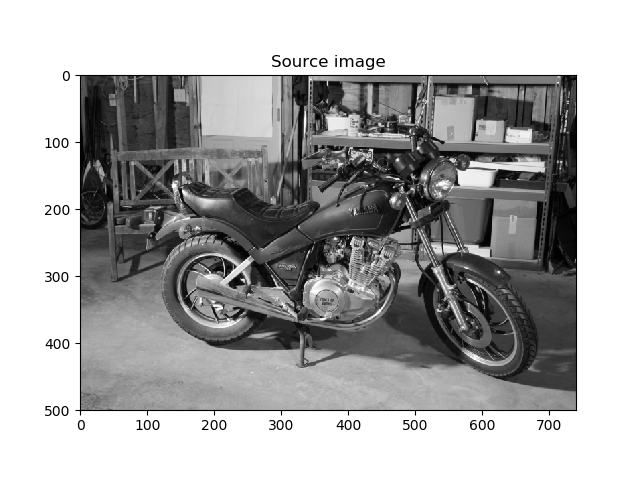
\includegraphics[width=0.55\textwidth,keepaspectratio]{daisy/bike_source.png}   
			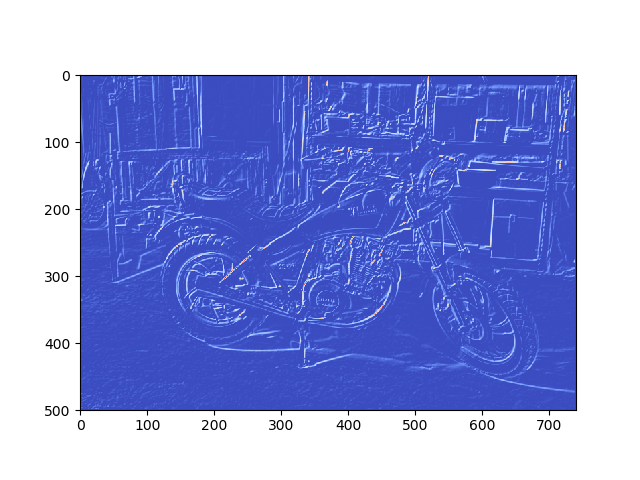
\includegraphics[width=0.55\textwidth,keepaspectratio]{daisy/bike_gradient.png}       
			\centering\caption{ Пример построения градиента изображения }
			\label{gradient_example}                           
		\end{figure}    
		
		Построенные карты градиентов подвергаются последовательному размытию с постепенным увеличением ядра гауссовского фильтра. Полученные карты называются свернутыми картами направлений (Convolved Orientation Maps, COM).
		
		\begin{figure}[H]
			\centering                             
			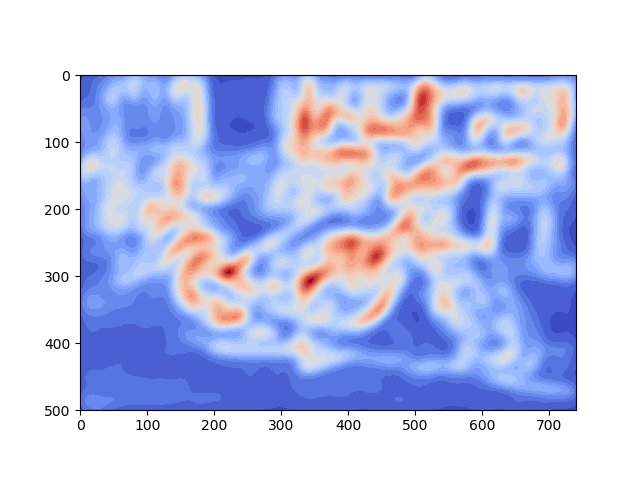
\includegraphics[width=0.6\textwidth,keepaspectratio]{daisy/bike_gradient_COM_1.png}   
			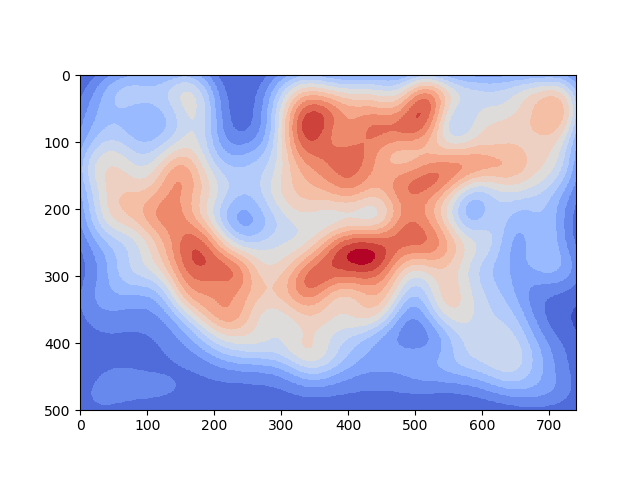
\includegraphics[width=0.6\textwidth,keepaspectratio]{daisy/bike_gradient_COM_2.png}       
			\centering\caption{ Пример COM с различными степенями размытия }
			\label{gradient_example}                           
		\end{figure}    
		
		Вычисление COM для изображения $I$ производится следующим образом:
		
		\begin{equation}\label{coms}
		G_o^\sigma = G^\sigma * \left(\dfrac{dI}{do}\right)^+ , \left(\dfrac{dI}{do}\right)^+ = max\left(\dfrac{dI}{do}, 0\right),
		\end{equation}
		\begin{tabular}{ rl }
			\quad \quad где 
			& $ G^\sigma $ -- ядро Гауссовского фильтра с стандартным отклонением $ \sigma $,\\
			& $o$ -- направление градиента.
		\end{tabular}\\
		
		Таким образом, получается набор карт градиента, каждая из которых с увеличением уровня размытия представляет собой все более обобщенную информацию о направлениях интенсивности исходного изображения. 
		
		Описанные операции выполняются один раз при начале работы алгоритма, полученные $T$ карт с различными уронями размытия далее используются для выборки результатов. 
		
		Выборка результатов для каждой точки $(u,v)$ изображения $I$ производится по следующей схеме:
		
		\begin{figure}[H]
			\centering                             
			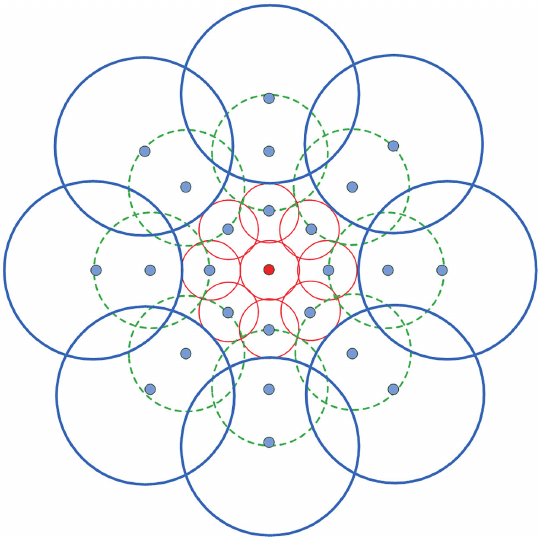
\includegraphics[width=0.5\textwidth,keepaspectratio]{daisy/DAISY-descriptor-structure.png}   
			\centering\caption{ Схема выборки значений из набора COM }
			\label{daisy_pattern}                           
		\end{figure}    
		
		Для каждой указанной на схеме точки выбираются значения COM, составляя очередной элемент дескриптора $h_\sigma(u,v)$. 
		
	    Каждый круг на схеме соответствует одной области выборки значений COM в его центральной точке. COM строятся для $H$ отдельных направлений, получая таким образом $H$ значений в точке.
		
		Точки выборки расположены $Q$ концентрическими кольцами вокруг центральной, для которой производится вычисление дескриптора, каждое кольцо задает $T \cdot H$ значений результата.
		
		Следовательно, общее число элементов дескриптора будет равно:
		\begin{equation}\label{elements_count}
		 D_s=(Q \cdot T+1)\cdot H.
		\end{equation}
		
		Вектор значений COM $h_\sigma(u,v)$ для точки $(u,v)$ задается следующим образом:
		\begin{equation}\label{single_vector}
		h_\sigma(u,v) = \left[G_1^\sigma(u,v), \dots, G_H^\sigma(u,v)\right]^T.
		\end{equation}
		Полученный вектор значений нормализуется. 
		
		Полный дескриптор для точки $(u_0,v_0)$ получается путем конкатенации всех нормализованных векторов значений COM $h_{\sigma i}(u,v)$, начиная с центральной точки:
		$$D(u_0,v_0) = [h_{\sigma 1}(u_0, v_0), h_{\sigma 1}(I_1(u_0, v_0, R_1)), \dots, h_{\sigma 1}(I_T(u_0, v_0, R_1),$$ 
		$$h_{\sigma 2}(I_1(u_0, v_0, R_2)), \dots, h_{\sigma 2}(I_T(u_0, v_0, R_2),$$
		$$\dots \dots$$
		$$h_{\sigma Q}(I_1(u_0, v_0, R_Q)), \dots, h_{\sigma Q}(I_T(u_0, v_0, R_Q)],$$
		\begin{tabular}{ rl }
			\quad \quad где 
			& $I_j(u, v, R)$ -- точка на расстоянии $R$ от $(u, v)$ в направлении\\
			& $j$ при числе направлений $T$.
		\end{tabular}\\
		
		При необходимости может производиться нормализация вектора значений дескриптора одним из следующих способов:
			\begin{enumerate}
				\item Нормализация отдельных векторов $h_\sigma(u,v)$;
				\item Полная нормализация вектора $D(u_0,v_0)$;
				\item Метод нормализации, применяемый в SIFT. После полной нормализации $D(u_0,v_0)$ вектор приводится к единичной сумме.
			\end{enumerate}
	
	
		Как можно видеть, описанный алгоритм отличается достаточно низкой вычислительной сложностью и простотой программной реализации. 
		
		Наиболее ресурсоемким этапом является построение диаграммы направленных градиентов и последовательное размытие COM. 
		
		Данные операции хорошо поддаются распараллеливанию или оптимизации путем замены свертки с крупным ядром последовательными свертками с ядрами меньшего размера, и выполняются один раз для всего изображения. Конфигурация паттерна выборки и методы нормализации влияют на производительность в незначительной степени, и могут варьироваться в широких пределах без серьезного повышения вычислительной сложности. 
	}
	\newpage
%   	\subsection{Программная реализация}{
%   		
%   		Алгоритм сшивки изображений для исследования был реализован на языке Python 3.7 с использованием библиотеки OpenCV 3.4.2. 
%   		
%   		Функция, осуществляющая процедуру совмещения, принимает на вход два изображения и тип используемого дескриптора. 
%   		Используются дескрипторы SIFT, SURF, ORB, BRIEF. Заметим, что алгоритмы SIFT и SURF являются патентованными, и не присутствуют в стандартной библиотеке OpenCV из-за лицензионных ограничений. Данные алгоритмы доступны в пакете xfeatures2d при использовании версии библиотеки, включающей неофициальные алгоритмы, opencv-contrib. Использование данных алгоритмов разрешается только в некоммерческих целях [\ref{cv docs}]. 
%   		
%   		Для вычисления дескрипторов производится преобразование исходных изображений в градации серого.
%   		
%   		\begin{lstlisting}[frame=single,language=Python,mathescape=true] 
%   		# convert the image to grayscale
%   		gray = cv2.cvtColor(image, cv2.COLOR_BGR2GRAY)
%   		\end{lstlisting}
%   		
%   		Производится поиск наборов особых точек при помощи выбранного дескриптора.
%   	
%   		\begin{lstlisting}[frame=single,language=Python,mathescape=true] 
%   		# detect keypoints in the image
%   		detector = cv2.FeatureDetector_create("SIFT")
%   		kps = detector.detect(gray)
%   		
%   		# extract features from the image
%   		extractor = cv2.DescriptorExtractor_create("SIFT")
%   		(kps, features) = extractor.compute(gray, kps)
%   		\end{lstlisting}
%   		
%   		Найденные наборы проверяются на совпадение дескрипторов методом knn. Полученные совпадения дополнпительно тестируются на предмет нахождения расстояния между точками в заданных пределах. Пары, прошедшие тест, используются для вычисления преобразования.
%   		
%   		\begin{lstlisting}[frame=single,language=Python,mathescape=true] 
%   		# compute the raw matches and initialize the list of actual
%   		# matches
%   		matcher = cv2.DescriptorMatcher_create("BruteForce")
%   		rawMatches = matcher.knnMatch(featuresA, featuresB, 2)
%   		matches = []
%   		
%   		# loop over the raw matches
%   		for m in rawMatches:
%   		# ensure the distance is within a certain ratio of each
%   		# other (i.e. Lowe's ratio test)
%   		if len(m) == 2 and m[0].distance < m[1].distance * ratio:
%   		matches.append((m[0].trainIdx, m[0].queryIdx))
%   		\end{lstlisting}
%   		
%   		После нахождения совпавших точек, по их наборам для каждого изображения вычисляется матрица проективного преобразования.
%   		Если совпавших опорных точек найдено меньше, чем четыре, проективное преобразование не может быть вычислено, и функция возвращает статус ошибки.
%   		
%   		\begin{lstlisting}[frame=single,language=Python,mathescape=true]
%   		 # compute the homography between the two sets of points
%   		(H, status) = cv2.findHomography(ptsA, ptsB, cv2.RANSAC,
%   		reprojThresh)
%   		\end{lstlisting}
%   		
%   		Построенная матрица проективного преобразования применяется ко второму входному изображению, трансформируя его до совпадения положений опорных точек.
%   		
%   		Исходное первое изображение и преобразованное второе записываются в одно результирующее. В зависимости от требуемых параметров, сложение может производиться с различными значениями альфа-канала, в том числе с выделением яркостью пересекающейся области либо одного из изображений в целях повышения наглядности.
%   		
%   		Функция возвращает результирующее изображение и отчет о работе алгоритма, включающий время выполнения и построенную матрицу проективного преобразования.
%   		
%   		Полный код функции представлен в приложении А.
%   	}
%\newpage


%------------------------------------------------
% Заключение
%------------------------------------------------

\titleformat{\section}{\large\bfseries\centering}{\thesection}{0.5em}{\MakeUppercase}
\titleformat{\subsection}[block]{\bfseries\hspace{1em}}{\thesubsection}{0.5em}{}

\newpage
\phantomsection
\addcontentsline{toc}{section}{Заключение}
\section*{Заключение}
{
    В ходе данной работы была собрана и проанализирована информация о существующих методах построения дескрипторов изображений. На основе существующего алгоритма DAISY был разработан алгоритм, потенциально обладающий высокой степенью устойчивости к пространственным преобразованиям исходного изображения.
    Разработанный алгоритм обладает набором параметров, позволяющих достаточно свободно варьировать точность и вычислительную сложность построения без изменения исходного кода, что позволяет эффективно адаптировать алгоритм к конкретным задачам. 
    Построенные дескрипторы можно использовать как в задачах распознавания, так и в задачах плотного сопоставления изображений. 
}

\newpage
\phantomsection
\addcontentsline{toc}{section}{Список использованных источников}
%------------------------------------------------
% Список литературы
%------------------------------------------------
\section*{Список использованных источников}
{
	\begin{enumerate}[label=\arabic*]
%	\item{Гонсалес Р., Вудс Р. Цифровая обработка изображений // М.: Техносфера. – 2005. – Т. 1072. – С. 2.}
	\item{Bres, S. Detection of interest points for image indexation [Текст] / S. Bres, J. M. Jolion // International Conference on Advances in Visual Information Systems. -- Springer, Berlin, Heidelberg, 1999. -- P. 427-435.}{\label{interest points}}	
	\item{Lowe, D. G. Distinctive image features from scale-invariant keypoints [Текст] / D. G. Lowe // International journal of computer vision. -- 2004. -- Vol. 60. -- I. 2. -- P. 91-110.}\label{lowe surf}
	\item{Tola, E. DAISY: A Fast Local Descriptor for Dense Matching [Текст] / E. Tola, V. Lepetit, P. Fua // IEEE Transactions on Pattern Analysis and Machine Intelligence. 2010. Vol. 32, num. 5  -- P. 815-830.}{\label{tola_paper}}	
	\item{Rublee, E. ORB: an efficient alternative to SIFT or SURF [Текст] / E. Rublee, D. Brando, J. Joestar // ICCV '11 Proceedings of the 2011 International Conference on Computer Vision. -- IEEE Computer Society Washington, DC, USA, 2011. -- P. 2564-2571. }\label{rublee orb}
	\item{Kong, H. A generalized Laplacian of Gaussian filter for blob detection and its applications [Текст] / H. Kong, H. C. Akakin, S. E. Sarma // IEEE transactions on cybernetics. -- IEEE Computer Society Washington, DC, USA, 2013. -- V. 43. -- I. 6. -- P. 1719-1733.}{\label{imagematching paper}}
	\item{Rekhil, M. A Survey on Image Feature Descriptors [Текст] / M. Rekhil, K. Sreekumar //  (IJCSIT) International Journal of Computer Science and Information Technologies, Vol. 5 (6) , 2014, -- P. 7668-7673.}{\label{surveyon}}
	\item{Funayama, R. Robust interest points detector and descriptor [Текст] / R. Funayama, H. Yanagihara //  Computer Vision and Image Understanding (CVIU), Vol. 110, No. 3 -- P. 346–359.}{\label{robust}}
	\item{Panchal, P. A Comparison of SIFT and SURF [Текст] / R. Funayama, H. Yanagihara //  International Journal of Innovative Research in Computer and Communication Engineering Vol. 1, Issue 2, April 2013 -- P. 287–302.}{\label{comparison}}

 	\item{OpenCV Documentation [Электронный ресурс] : официальная документация библиотеки OpenCV. / Intel Corporation, Willow Garage Inc., Itseez Ltd. -- Электрон. дан. -- 2019. -- URL: \\https://docs.opencv.org (дата обращения: 20.11.2019). }{\label{cv docs}}
 	\item{Scikit-image Documentation [Электронный ресурс] : официальная документация библиотеки scikit-image. / The scikit-image team. -- Электрон. дан. -- 2019. -- URL: \\https://scikit-image.org/docs/stable/ (дата обращения: 25.11.2019). }{\label{skimg docs}}
	\item {Karami, E. Image Matching Using SIFT, SURF, BRIEF and ORB: Per-\\formance Comparison for Distorted Images [Электронный ресурс] / E. Karami, S. Prasad, M. Shehata // Journal of Visual Communication and Image Representation -- 2015. -- Электрон. дан. -- URL:\\ https://www.sciencedirect.com/science/article/pii/S1047320315002230\quad (дата обращения: 03.12.2019).}
	\item {Xue, B. A DAISY descriptor based multi-view stereo method for large-scale scenes [Электронный ресурс] / B. Xue, L. Cao // Advances in Intelligent Systems and Computing -- 2015. -- Электрон. дан. -- URL:\\ https://doi.org/10.1016/j.jvcir.2015.11.007\quad (дата обращения: 06.12.2019).}
	\item {Tola, E. DAISY: An Efficient Dense Descriptor Applied to Wide-Baseline Stereo [Электронный ресурс] / E. Tola //IEEE Xplore Digital Library -- 2014. -- Электрон. дан. -- URL:\\ https://ieeexplore.ieee.org/document/4815264\quad (дата обращения: 05.12.2019).}
\end{enumerate}


%--------------------------------
% Приложения. Коды программ и.т.д.
%--------------------------------
\newpage
\phantomsection
%\addcontentsline{toc}{section}{Приложение А Код программы}

%\section*{Приложение А}
%{
%	\begin{center}
%	\textbf{Код программы}
%	\end{center}
%%	Файл stitching.py:
%%	\lstinputlisting[language=python,mathescape=true]{./src/stitching.py}
%	\newpage
%	%\lstinputlisting[language=python,mathescape=true]{./src/test.py}
%}

\end{document}
